\documentclass[9pt]{beamer}

%\usepackage{tikz}
\usepackage{amsmath}
\usepackage{amsfonts}
\usepackage{amssymb}
\usepackage{algorithm2e}
\usepackage{color, colortbl}
\usepackage{enumerate}
\usepackage{arydshln}
\usepackage{multirow}

\renewcommand{\figurename}{Fig}
\usetheme{uha}



%\theoremstyle{plain}
%  \newtheorem{theorem}{Theorem}
%  \newtheorem{lemma}{Lemma}
\newtheorem{corrolary}{Corollary}
\newtheorem{claim}{Claim}
\newtheorem{proposition}{Proposition}
\newtheorem{property}{Property}
%  \newtheorem{fact}{Fact}
%\theoremstyle{definition}
%  \newtheorem{definition}{Definition}
%  \newtheorem{example}{Example}
%\theoremstyle{remark}
\newtheorem{remark}{Remark}
\newtheorem{proviso}{Proviso}


\newcommand{\ccr}[1]{{\color{red}#1}}
\newcommand{\ccb}[1]{{\color{blue}#1}}
\newcommand{\ccp}[1]{{\color{purple}#1}}
\newcommand{\ccm}[1]{{\color{magenta}#1}}
\newcommand{\cco}[1]{{\color{orange}#1}}
\newcommand{\ccy}[1]{{\color{yellow}#1}}
\newcommand{\ccl}[1]{{\color{lime}#1}}
\newcommand{\ccc}[1]{{\color{cyan}#1}}
\newcommand{\ccg}[1]{{\color{gray}#1}}
\newcommand{\ccpk}[1]{{\color{pink}#1}}
\newcommand{\ccov}[1]{{\color{olive}#1}}



\begin{document}

%%//////////////////////////////////////////////////////////////////////////////////////////////%%1

\title{Clustering}
\subtitle{K-means}
\author{Haotian Wang and Yiyan Li}
\institute{School of Software, Shanghai Jiao Tong University}
\date{\hspace{2em}}
\frame{
	\titlepage
}
%%//////////////////////////////////////////////////////////////////////////////////////////////%%
\section{Introduction to clustering}
\begin{frame}
	\frametitle{Clustering}
	\begin{definition}
		A cluster is a collection of objects which are “similar” between them and are “dissimilar” to the objects belonging to other clusters.
	\end{definition}
	\begin{definition}
		Clustering is the algorithm that recognizes clusters from a given data set.
	\end{definition}
	\pause
	Part of common application domains in which the clustering problem arises are as follows:
	\begin{itemize}
		\item Multimedia Data Analysis
		\item Responding to public health crises
		\item Intermediate Step for other fundamental data mining problems
		\item Intelligent Transportation
	\end{itemize}
\end{frame}

%%//////////////////////////////////////////////////////////////////////////////////////////////%%1
\section{K-means Algorithm}
%%//////////////////////////////////////////////////////////////////////////////////////////////%%
\begin{frame}
	\frametitle{K-means}
	The \ccp{k-means clustering} problem is one of the oldest and most important questions in all of computational geometry.
	\par Given an integer $k$ and a set of $n$ data points in $\mathbb{R}^{d}$, the goal of this problem is to choose \ccp{$k$ centers} so as to \ccp{minimize the total squared distance between each point and its closest center}.
	\par The most common K-means algorithm was first proposed by \ccp{Stuart Lloyd} of Bell Labs in 1957.

\end{frame}
%%//////////////////////////////////////////////////////////////////////////////////////////////%%
\begin{frame}
	\frametitle{K-means}
	The objective function to minimize is the \ccp{within-cluster sum of squares} (WCSS) cost:
	$$Cost(C_{1:k}, c_{1:k}) = \sum_{i=1}^{k} \sum_{x \in C_i } {\left\lVert x - c _i \right\rVert }^2  $$
	where $c_i$ is the \ccp{centroid} of cluster
	\begin{definition}
		\ccp{Cluster centroid} is the \ccp{middle} of a cluster.
		\par A centroid is a vector that contains one number for each variable, where each number is the mean of a variable for the observations in that cluster.
		\par The centroid can be thought of as the multi-dimensional average of the cluster.
	\end{definition}
\end{frame}
%%//////////////////////////////////////////////////////////////////////////////////////////////%%
\begin{frame}
	\frametitle{K-means}
	\begin{lemma}
		Let $C$ be a cluster of points with its mean to be $\mu$, and let $c$ to be and arbitrary point.Then $\sum_{x \in C}{\left\lVert x - c\right\rVert}^2 = \sum_{x \in C}{\left\lVert x - \mu\right\rVert}^2 + \left\lvert C \right\rvert \cdot {\left\lVert c - \mu\right\rVert}^2 $
	\end{lemma}
	So we denote that:
	\begin{equation*}
		\begin{split}
			Cost(C_{1:k}, c_{1:k}) & = \sum_{i=1}^{k} \sum_{x \in C_i } {\left\lVert x - c _i \right\rVert }^2 \\
			& = \sum_{i=1}^{k} (\sum_{x \in C_i} {\left\lVert x - \mu_i\right\rVert}^2 + \left\lvert C_i \right\rvert \cdot {\left\lVert c_i - \mu_i\right\rVert}^2) \\
			& = Cost(C_{1:k}, mean(C_{1:k})) + \sum_{i=1}^{k} {\left\lvert C_i\right\rvert }\cdot {\left\lVert c_i - \mu_i\right\rVert }^2
		\end{split}
	\end{equation*}
\end{frame}
%%//////////////////////////////////////////////////////////////////////////////////////////////%%
\begin{frame}
	\frametitle{Toward a K-means Algorithm}
	The k-means algorithm \ccp{iteratively} calculates the sum of distance within a cluster and updates the partition.
	\begin{enumerate}
		\item Arbitrarily choose and initial \ccb{$k$} centroids \ccb{$\mathcal{C} = \{c_1, c_2 \dots c_k\}$}
		\item For each $i \in \{1, 2 \dots k\}$, set the cluster $C_i$ to be the set of points that are \ccp{closer} to $c_i$ than they are to $c_j$ for all $j \neq i$
		\item For each $i \in \{1, 2 \dots k\}$, set $c_i$ to be the center of all points in $C_i$ where \ccb{$c_i = \frac{1}{\left\lvert C_i \right\rvert }\sum_{x \in C_i} x $}
		\item Repeat Step 2 and Step 3 until \ccb{$\mathcal{C}$} no longer changes.
	\end{enumerate}
\end{frame}

\begin{frame}
	\frametitle{Toward a K-means Algorithm}
	Iteration = 1
	\centerline{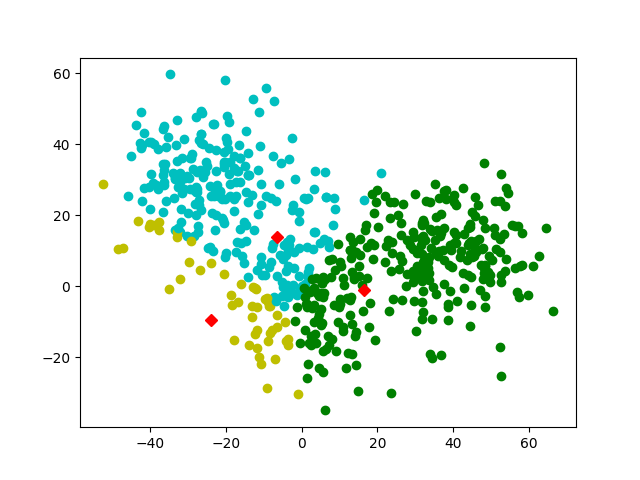
\includegraphics[width=0.65\textwidth]{figures/iteration1.png}}

\end{frame}

\begin{frame}
	\frametitle{Toward a K-means Algorithm}
	Iteration = 2
	\centerline{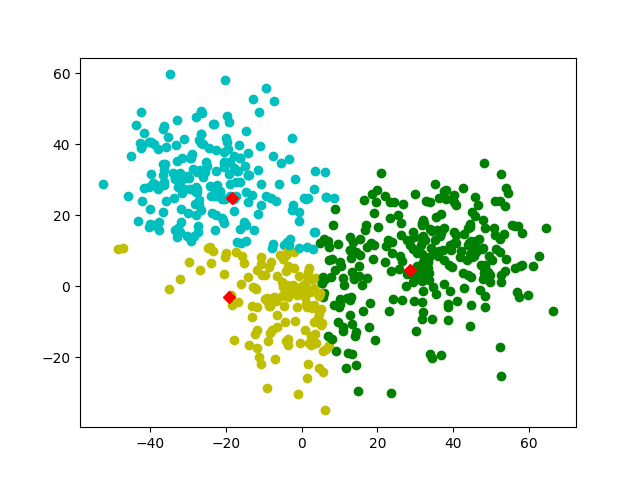
\includegraphics[width=0.65\textwidth]{figures/iteration2.png}}

\end{frame}

\begin{frame}
	\frametitle{Toward a K-means Algorithm}
	Iteration = 3
	\centerline{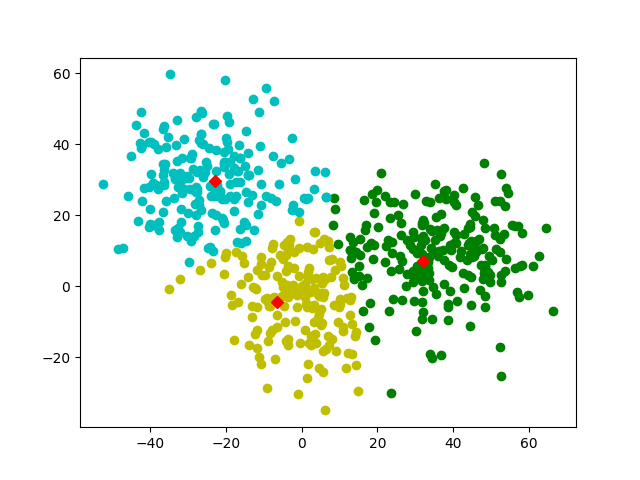
\includegraphics[width=0.65\textwidth]{figures/iteration3.png}}

\end{frame}

\begin{frame}
	\frametitle{Toward a K-means Algorithm}
	Iteration = 4
	\centerline{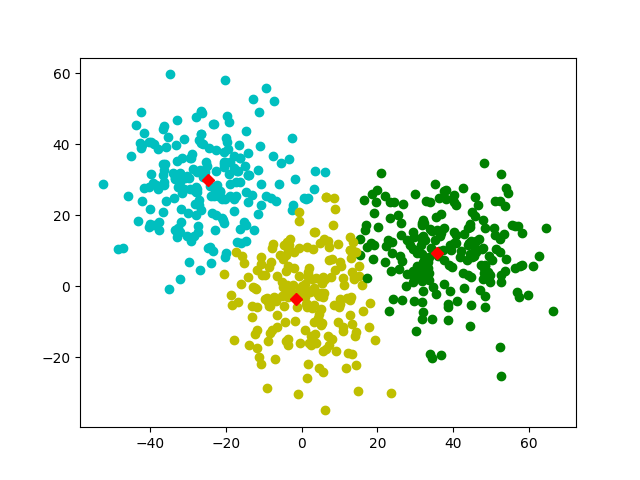
\includegraphics[width=0.65\textwidth]{figures/iteration4.png}}

\end{frame}

\begin{frame}
	\frametitle{Toward a K-means Algorithm}
	Iteration = 5
	\centerline{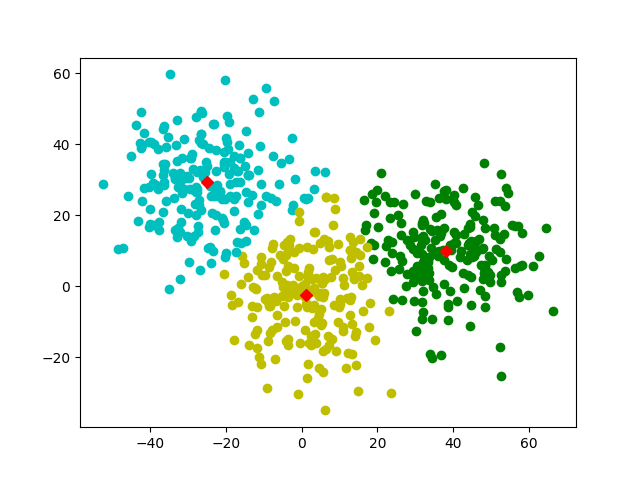
\includegraphics[width=0.65\textwidth]{figures/iteration5.png}}

\end{frame}

\begin{frame}
	\frametitle{Toward a K-means Algorithm}
	Iteration = 6
	\centerline{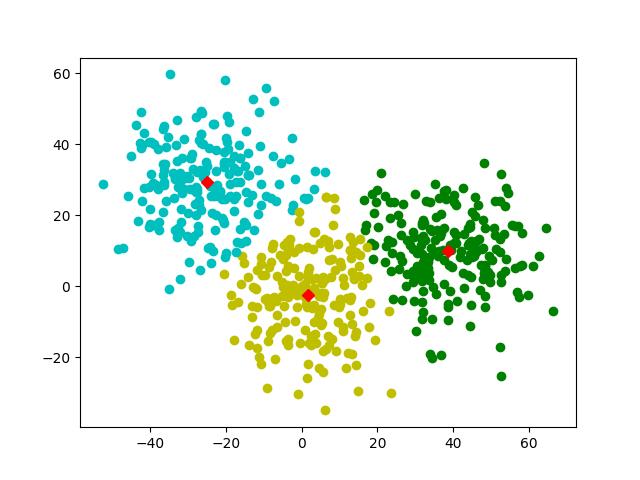
\includegraphics[width=0.65\textwidth]{figures/iteration6.png}}

\end{frame}

\begin{frame}
	\frametitle{Convergence of K-means}
	\begin{proof}
		During the course of the k-means algorithm, the cost monotonically decreases.
	\end{proof} \pause
	Let \ccb{$c_1^{(t)} \dots c_k^{(t)}, C_1^{(t)} \dots C_k^{(t)}$} denote the cetnroids and clusters at the start of $t^{th}$ iteration of K-means.
	\pause
	\par The first step of the iteration assigns each point to its nearest center, therefore:
	$$Cost(C_{1:k}^{(t+1)}, c_{1:k}^{(t)}) \leq Cost(C_{1:k}^{(t)}, c_{1:k}^{(t)})$$
	\pause
	On the second step, each cluster re-centered at its mean. By lemma above:
	$$Cost(C_{1:k}^{(t+1)}, c_{1:k}^{(t+1)}) \leq Cost(C_{1:k}^{(t+1)}, c_{1:k}^{(t)})$$

\end{frame}
%%//////////////////////////////////////////////////////////////////////////////////////////////%%
\begin{frame}
	\frametitle{Time Complexity}
	\begin{proof}
		Naive K-means algorithm's time complexity is \ccb{$O(kni)$}
	\end{proof} \pause
	In each iteration there are such steps:
	\begin{itemize}
		\item Distance calculation: To calculate the distance from a point to the centroid, we can use the squared Euclidean proximity function, which is thought to be $O(1)$
		\item Comparisons betweeen distances.
		\item Centroid calculation.
	\end{itemize}
\end{frame}

\begin{frame}
	\frametitle{Time Complexity}
	\begin{proof}
		Naive K-means algorithm's time complexity is \ccb{$O(kni)$}
	\end{proof}
	\par So the total number of operations in one iteration is:
	\begin{equation*}
		\begin{split}
			C &=  distance\ calculation + comparisons + centroids\ calculation\\
			& = k * n * O(1) + (k-1) * n * O(1) + k * n * O(1) \\
			& = O(kn)
		\end{split}
	\end{equation*}
	where k denotes the number of clusters, n denotes the count of data vectors and d denotes vector dimension.
	\par And the whole process takes $i$ iterations in total so the time complexity of K-means algorithm is \ccb{$O(kni)$}.
\end{frame}

\begin{frame}
	\frametitle{Drawback of K-means}

	

\end{frame}

%% Lee begins here
%% avoid redundant
%%//////////////////////////////////////////////////////////////////////////////////////////////%%
\begin{frame}
	\frametitle{Avoid redundant computation}
	There are $n$ data points in $\mathbb{R}^ d$ space and $k$ clusters for partition, each iteration involves $n * k$ distance computations.\par
	There exist many unnecessary calculations in the process of iteration! \par
	\pause
	\par If a point is \ccp{far away from a centroid}, it is not necessary to calculate the exact distance between the point and the centroid in order to know that the point should not be assigned to this centroid.\par
 Conversely, \ccp{if a point is much closer to one center than to any other}, calculating exact distances is not necessary to know that the point should be assigned to the first center. 


\end{frame}

%%//////////////////////////////////////////////////////////////////////////////////////////////%%
\begin{frame}
	\frametitle{Avoid redundant computation}
	The key idea is to \ccp{bound on data point} to cluster centroid distance and use \ccp{triangle inequality} to avoid redundant computations of distance between data points and cluster centroids.
	\begin{lemma}
	Triangle inequality: For any 3 points $x, y, z$, $d(x,z) \le d(x, y) + d(y, z)$.
	\end{lemma} 
The only black box property of any distance metrics.
\end{frame}

%%//////////////////////////////////////////////////////////////////////////////////////////////%%
\begin{frame}
	\frametitle{Avoid redundant computation}
	\begin{lemma}
Let x be a point and let b and c be centers. If $d(b, c) \ge 2d(x,b)$ then $d(x,c) \ge d(x,b)$.
\end{lemma}
\begin{proof}
Use triangle inequality, $d(b,c) - d(x,b)\le d(x,c)$. And bring in $d(b, c) \ge 2d(x,b)$, we can get the conclusion.
\end{proof}
\pause
\begin{lemma}
Let x be a point and let b and c be centers. $d(x,c) \ge max(0, d(x,b)-d(b,c))$.
\end{lemma}
\begin{proof}
Use triangle inequality $d(x,c) \ge d(x,b)-d(b,c)$, with $d(x,c) \ge 0$, we can get the conclusion.
\end{proof}
\end{frame}

%%//////////////////////////////////////////////////////////////////////////////////////////////%%
\begin{frame}
\frametitle{Avoid redundant computation}
	\begin{corollary}
if $\frac{1}{2}d(c, s) \ge d(x,c)$ then $d(x, s) \ge d(x, c)$, and we \ccp{don't need to compute $d(x,s)$.} 
\end{corollary}
\pause
\begin{corollary}
Suppose that we don't know $d(x,c)$ exactly, and we do know an upper bound u such that $u \ge d(x,c)$: For any other possible choice, \ccp{we only need to compute $d(x, c), d(x, s)$ iff $u > \frac{1}{2}d(c, s)$ .}
\end{corollary}

\end{frame}

%%//////////////////////////////////////////////////////////////////////////////////////////////%%
\begin{frame}
	\frametitle{Avoid redundant computation}
	\begin{corollary}
Suppose that $u \le \frac{1}{2}d(c, s)$ for any possible s, all distance calculations for x can be avoided. 
\end{corollary}
\end{frame}

%%//////////////////////////////////////////////////////////////////////////////////////////////%%
\begin{frame}
\frametitle{Avoid redundant computation}
Let $x$ be any data point, let $c$ be any center, let s become previous version of same center. Suppose that in the previous iteration we knew a lower bound g such that $d(x, s) \ge g$ Then we can infer a lower bound h for current iteration: \par
\begin{equation*}	
	d(x, c) \ge max\{0, d(x,s)-d(s,c)\} \ge max\{0, g-d(s,c)\} = h
	\end{equation*}
\pause
\begin{claim}
\ccp{If center moved a small distance$(d(s,c)$ is small}, the lower bound only make a small move.
\end{claim}
\end{frame}



%%//////////////////////////////////////////////////////////////////////////////////////////////%%
\begin{frame}
	\frametitle{Augmentation detail}
 We use $u(x)$ to represent upper bound of distance between a given point $x$ and its currently assigned center $c$. $l(x,c^{\prime})$ is the lower bound on the distance between x and some other center $c^{\prime}$.\par
\begin{claim}
If $u(x) \le l(x,c^{\prime}) $, we don't need to calculate $d(x,c), d(x, c^{\prime})$. \par
\end{claim}
\end{frame}

%%//////////////////////////////////////////////////////////////////////////////////////////////%%
\begin{frame}
	\frametitle{Augmentation preparation}
 Initially, we set $l(x,c)=0$ for each point x and center c. Then assign each x to its closest initial center.\par
Each time $d(x,c)$ is computed, set $l(x,c)=d(x,c)$. At last, set upper bounds $u(x) = min_c(d(x,c))$.

\end{frame}

%%//////////////////////////////////////////////////////////////////////////////////////////////%%
\begin{frame}
	\frametitle{Augmentation detail}

Then repeate this until convergence.
\begin{enumerate}
\item For all centers c and $c^{\prime}$, compute $d(c, c^{\prime})$. Set $s(c) = \frac{1}{2}min_{c \ne c^{\prime}}d(c,c^{\prime})$.
\item \ccp{Identify all points x such that $u(x) \le s(c(x))$. }
\item For each pair of remaining x and c, which satisfy: i) $c \ne c(x)$ and ii) $u(x) > l(x,c)$ and \ccp{iii) $u(x) > \frac{1}{2}d(c(x), c)$}: 
\begin{enumerate}
\item If $r(x) = true$, compute $d(x,c(x))$ and assign $r(x)=false$. \ccp{Otherwise, $d(x,c(x)) = u(x).$ }
\item \ccp{If $d(x,c(x))> l(x,c)$ or $d(x,c(x)) > \frac{1}{2}d(c(x), c)$}, then compute $d(x,c)$ and decide if swap c for x. 
\end{enumerate}

\end{enumerate}
\end{frame}

%%//////////////////////////////////////////////////////////////////////////////////////////////%%
\begin{frame}
	\frametitle{Augmentation detail}
\begin{enumerate}
\setcounter{enumi}{3} 
\item For each center c, compute centroid, store in m(c).
\item For each  pair of x and c, set $l(x,c) = max(l(x,c) - d(c,m(c)), 0)$
\item For each point x, set $u(x) = u(x) + d(m(c(x)), c(x))$
\item For each point x, set $r(x) = True$
\item Really replace c by m(c)
\end{enumerate}
\end{frame}

%%//////////////////////////////////////////////////////////////////////////////////////////////%%
\begin{frame}
	\frametitle{Discussion}
Compared to naive K-means++ algorithm, in 6 typical benchmark, using this optimazation speeds up algorithms from $ 11.3 \times$ to $  351 \times$.
\end{frame}

%%//////////////////////////////////////////////////////////////////////////////////////////////%%
\begin{frame}
	\frametitle{Relax the restriction}
Another contribution helps reduce the iteration cost to $n * k^{\prime}$ ($k^{\prime} << k$) by generating \ccp{candidate cluster list (CCL)} of size $k^{\prime}$ for each data point. \par
This augmentation makes trade-off between loss function and running time and relaxes the previous algorithm's restrictions.Their target:
\begin{itemize}
\item \textbf{For convergence time:} $T^{\prime} < T$
\item \textbf{For loss:} $E^{\prime} \le E \space $ or $ \space E^{\prime} \overset{marginally}{>} E$
\end{itemize}
\end{frame}

%%//////////////////////////////////////////////////////////////////////////////////////////////%%
\begin{frame}
	\frametitle{How it works}
Consider a data point p1 and cluster centroids represented as $c_1$, $c_2$..., $c_k$. We assume that $k^{\prime} << k $ and there is a candidate cluster list for $p_1$.\par
\pause
 If we run K-means for second iteration, $p_1$ will compute distance to all k centroids. After second iteration, there are two possible cases:
\begin{enumerate}
\item The list do not change but only members'ranking changes.
\item Several members of the centroids in the previous list are replaced with other centroids which were not in the list.
\end{enumerate}
\textbf{In real world data rarely makes case 2 happen}! That is, the set of top few closest centroids for a data point \textbf{remains almost unchange}.
\end{frame}

%%//////////////////////////////////////////////////////////////////////////////////////////////%%
\begin{frame}
	\frametitle{Augmentation analysis}
Overhead analysis:
\begin{itemize}
\item \textbf{Computation overhead:} $O(nklog(k))$ for creating CCL at first. We have to compute the distance to each cluster's centroid for each point and sort them to create CCL. 
\item \textbf{Memory overhead:}$ O(nk^{\prime})$ to maintain CCL.
\end{itemize}
\end{frame}

%%//////////////////////////////////////////////////////////////////////////////////////////////%%
\begin{frame}
	\frametitle{Choose a proper K}
\ccp{Use a range of set}: We choose a set of K and compare their performance. In this set, we need to choose k \ccp{significantly smaller than the number of objects in the data sets and let it be resonably large based on this}.\par


\end{frame}

%%//////////////////////////////////////////////////////////////////////////////////////////////%%
\begin{frame}
	\frametitle{Choose a proper K}
\ccp{statistical measures}: There are several statistical measures available for selecting K. \ccp{They are calculated with certain assumptions about the underlying distribution of the data.} \par
e.g. The Bayesian information criterion is calculated on data sets which are constructed by a set of \textbf{Gaussian distributions}. \par
\end{frame}

%%//////////////////////////////////////////////////////////////////////////////////////////////%%
\begin{frame}
	\frametitle{Choose a proper K}
\ccp{visualization}: Visual verification is applied widely because of its simplicity and explanation possibilities. In my own practice, I usually use PCA or other methods to draw points on a planar graph to check how many clusters exist in Machine Learning course's project. But it has many restrictions. e.g. The application of
visualization techniques implies a data distribution continuity in the expected clusters. In fact, Visual examples are often used to illustrate the drawbacks of an algorithm. \par

\end{frame}

\section{Key properties}
%%//////////////////////////////////////////////////////////////////////////////////////////////%%
\begin{frame}
	\frametitle{Discussion}

\end{frame}

%%//////////////////////////////////////////////////////////////////////////////////////////////%%
\begin{frame}
	\frametitle{Discussion}

\end{frame}


\section{Application}
%%//////////////////////////////////////////////////////////////////////////////////////////////%%
\begin{frame}
	\frametitle{Discussion}

\end{frame}

%%//////////////////////////////////////////////////////////////////////////////////////////////%%
\begin{frame}
	\frametitle{Discussion}

\end{frame}

%%//////////////////////////////////////////////////////////////////////////////////////////////%%
\begin{frame}
	\frametitle{Discussion}

\end{frame}

%%//////////////////////////////////////////////////////////////////////////////////////////////%%
\begin{frame}
	\frametitle{Discussion}

\end{frame}

%%//////////////////////////////////////////////////////////////////////////////////////////////%%
\begin{frame}
	\frametitle{Discussion}

\end{frame}

\section{Conclusion}
%%//////////////////////////////////////////////////////////////////////////////////////////////%%
\begin{frame}
	\frametitle{Discussion}

\end{frame}


\end{document}
